\documentclass[aspectratio=169,10pt]{beamer}

% ============================================================
% OmniCast - Joint Project Defense Presentation Slide Deck
% Courses: PRN232 (Back-End) & PRM393 (Mobile Client)
% FPTU Quy Nhon AI Campus - FU Cahata | Mentor: Mr. Huỳnh Vang
% ============================================================

\usepackage{fontspec}
\setmainfont{Arial}
\setsansfont{Arial}
\setmonofont{Consolas}

\usepackage{tikz}
\usetikzlibrary{calc,positioning,arrows.meta,shapes.geometric,fit,backgrounds}
\usepackage{booktabs}
\usepackage{tabularx}
\usepackage{xcolor}
\usepackage{url}
\usepackage{listings}
\usepackage{tcolorbox}
\tcbuselibrary{skins,breakable}

% ---------- OmniCast Cinema Dark Color Scheme ----------
\definecolor{omniDark}{HTML}{0B132B}
\definecolor{omniCard}{HTML}{16203A}
\definecolor{omniDeep}{HTML}{070C1B}
\definecolor{omniCyan}{HTML}{00E5FF}
\definecolor{omniBlue}{HTML}{38BDF8}
\definecolor{omniTeal}{HTML}{14B8A6}
\definecolor{omniPurple}{HTML}{A78BFA}
\definecolor{omniAmber}{HTML}{FBBF24}
\definecolor{omniGreen}{HTML}{34D399}
\definecolor{omniSlate}{HTML}{94A3B8}
\definecolor{omniBorder}{HTML}{2A3756}
\definecolor{omniLight}{HTML}{F8FAFC}

% ---------- Beamer Theme Settings ----------
\setbeamercolor{background canvas}{bg=omniDark}
\setbeamercolor{normal text}{fg=omniLight}
\setbeamercolor{title}{fg=white}
\setbeamercolor{subtitle}{fg=omniCyan}
\setbeamercolor{author}{fg=omniSlate}
\setbeamercolor{date}{fg=omniSlate}
\setbeamercolor{frametitle}{fg=white,bg=omniDark}
\setbeamercolor{structure}{fg=omniCyan}
\setbeamercolor{item}{fg=omniCyan}

\setbeamertemplate{navigation symbols}{}

% ---------- Custom Header & Footer ----------
\setbeamertemplate{headline}{
  \leavevmode
  \begin{tikzpicture}[remember picture, overlay]
    \fill[omniDeep] (current page.north west) rectangle ($(current page.north east) + (0,-10mm)$);
    \draw[omniBorder, line width=0.5pt] ($(current page.north west) + (0,-10mm)$) -- ($(current page.north east) + (0,-10mm)$);
    \node[anchor=west, text=omniCyan, font=\scriptsize\bfseries] at ($(current page.north west) + (8mm,-5mm)$) {OMNICAST};
    \node[anchor=west, text=omniSlate, font=\scriptsize] at ($(current page.north west) + (26mm,-5mm)$) {$\vert$ \ \insertsectionhead};
    \node[anchor=east, text=omniSlate, font=\tiny] at ($(current page.north east) + (-8mm,-5mm)$) {FPTU QUY NHON AI CAMPUS --- FU CAHATA $\bullet$ MENTOR: MR. HUỲNH VANG};
  \end{tikzpicture}
  \vspace{8mm}
}

\setbeamertemplate{footline}{
  \leavevmode
  \begin{tikzpicture}[remember picture, overlay]
    \fill[omniDeep] (current page.south west) rectangle ($(current page.south east) + (0,6mm)$);
    \draw[omniBorder, line width=0.5pt] ($(current page.south west) + (0,6mm)$) -- ($(current page.south east) + (0,6mm)$);
    \node[anchor=west, text=omniSlate, font=\tiny] at ($(current page.south west) + (8mm,3mm)$) {Nguyễn Bình An $\cdot$ Trần Thanh Sơn $\cdot$ Nguyễn Vĩnh Phú $\cdot$ Đồng Hoàng Nguyên};
    \node[anchor=center, text=omniSlate, font=\tiny] at ($(current page.south) + (0,3mm)$) {FPTU Quy Nhon AI Campus --- FU Cahata $\vert$ PRN232 \& PRM393};
    \node[anchor=east, text=omniCyan, font=\tiny\bfseries] at ($(current page.south east) + (-8mm,3mm)$) {\insertframenumber{} / \inserttotalframenumber{}};
  \end{tikzpicture}
}

\setbeamertemplate{frametitle}{
  \vspace*{2mm}
  \begin{beamercolorbox}[wd=\paperwidth,ht=4ex,dp=1ex,leftskip=8mm]{frametitle}
    {\large\bfseries\insertframetitle}
    \ifx\insertframesubtitle\@empty\else
      \ \ {\footnotesize\color{omniSlate}--- \insertframesubtitle}
    \fi
  \end{beamercolorbox}
}

% ---------- Custom Visual Card Command using Native Beamer Blocks ----------
\setbeamertemplate{blocks}[rounded][shadow=true]

\newcommand{\card}[4]{%
  \begingroup
  \setbeamercolor{block title}{bg=omniDeep,fg=#2}%
  \setbeamercolor{block body}{bg=omniCard,fg=omniLight}%
  \begin{block}{\scriptsize\bfseries #3}%
    \scriptsize #4%
  \end{block}%
  \endgroup
}

% ---------- Title Information ----------
\title{OMNICAST}
\subtitle{Enterprise Media \& Broadcast Intelligence Network}
\author{Nguyễn Bình An $\cdot$ Trần Thanh Sơn $\cdot$ Nguyễn Vĩnh Phú $\cdot$ Đồng Hoàng Nguyên}
\institute{FPTU Quy Nhon AI Campus --- FU Cahata $\bullet$ Mentor: Mr. Huỳnh Vang}
\date{Fall Semester 2026 (FA26)}

\begin{document}

% ============================================================
% SLIDE 1: Title Slide (Full Bleed Cinema Dark)
% ============================================================
{
\setbeamertemplate{headline}{}
\setbeamertemplate{footline}{}
\begin{frame}[plain]
  \begin{tikzpicture}[remember picture, overlay]
    \fill[omniDeep] (current page.north west) rectangle (current page.south east);
    \draw[omniCyan!25, line width=0.8pt, dashed] ($(current page.north west) + (10mm,-10mm)$) rectangle ($(current page.south east) + (-10mm,10mm)$);
    \draw[omniBorder, line width=1.2pt] ($(current page.north west) + (12mm,-12mm)$) rectangle ($(current page.south east) + (-12mm,12mm)$);
    \fill[omniCyan] ($(current page.north west) + (12mm,-12mm)$) circle (2.5pt);
    \fill[omniCyan] ($(current page.north east) + (-12mm,-12mm)$) circle (2.5pt);
    \fill[omniCyan] ($(current page.south west) + (12mm,12mm)$) circle (2.5pt);
    \fill[omniCyan] ($(current page.south east) + (-12mm,12mm)$) circle (2.5pt);
  \end{tikzpicture}

  \begin{center}
    \vspace*{-5mm}
    {\scriptsize\bfseries\color{omniCyan}FPT UNIVERSITY $\bullet$ FPTU QUY NHON AI CAMPUS --- FU CAHATA}\\[1.5mm]
    {\tiny\color{omniSlate}\bfseries FINAL CAPSTONE DEFENSE \& PROJECT PRESENTATION (FALL 2026)}\\[3mm]

    {\Huge\bfseries\color{white}OMNI\textcolor{omniCyan}{CAST}}\\[1mm]
    {\large\bfseries\color{omniSlate}Enterprise Media, Real-Time LiveStream \& Broadcast Intelligence Network}\\[2.5mm]
    
    {\color{omniBorder}\rule{0.72\linewidth}{1pt}}\\[2.5mm]

    
\begin{tikzpicture}
      \node[draw=omniBlue, fill=omniCard, rounded corners=3pt, line width=0.8pt, inner sep=4pt] (b1) at (-3.4,0) {
        \textbf{\scriptsize\color{white}PART 1: PRN232} \ \textcolor{omniSlate}{\tiny$\vert$} \ \textsf{\scriptsize\color{omniBlue}Back-End, gRPC \& Next.js 15 (33 Routes)}
      };
      \node[draw=omniPurple, fill=omniCard, rounded corners=3pt, line width=0.8pt, inner sep=4pt] (b2) at (3.4,0) {
        \textbf{\scriptsize\color{white}PART 2: PRM393} \ \textcolor{omniSlate}{\tiny$\vert$} \ \textsf{\scriptsize\color{omniPurple}Flutter Mobile App (31 Screens \& Live Studio)}
      };
    \end{tikzpicture}
    \vspace{2.5mm}

    
\begin{tikzpicture}
      \node[text=omniGreen, font=\tiny\bfseries] at (-4.2,0) {$\checkmark$ 142,897 Physical LOC};
      \node[text=omniCyan, font=\tiny\bfseries] at (0,0) {$\checkmark$ 482/482 Automated Tests PASS (100\%)};
      \node[text=omniAmber, font=\tiny\bfseries] at (4.4,0) {$\checkmark$ WebRTC WHIP/WHEP + Socket.IO /live};
    \end{tikzpicture}
    \vspace{2.5mm}

    {\scriptsize\color{omniSlate}Mentor / Supervisor: \textbf{\color{omniAmber}Thầy Huỳnh Vang (Mr. Huỳnh Vang)}}\\[1.5mm]
    {\scriptsize\color{white}\textbf{Nguyễn Bình An} \ $\bullet$ \ \textbf{Trần Thanh Sơn} (\texttt{QE170080}) \ $\bullet$ \ \textbf{Nguyễn Vĩnh Phú} (\texttt{QE180136}) \ $\bullet$ \ \textbf{Đồng Hoàng Nguyên}}\\[1mm]
    {\tiny\color{omniCyan}FPTU Quy Nhon AI Campus --- FU Cahata $\bullet$ October 2026}
  \end{center}
\end{frame}
}

% ============================================================
% SLIDE 2: Project Team & Mentorship (FPTU Quy Nhon AI Campus - FU Cahata)
% ============================================================
\section{Overview \& Team}
\begin{frame}{Project Team \& Academic Mentorship}{FPTU Quy Nhon AI Campus --- FU Cahata $\bullet$ Mentor: Thầy Huỳnh Vang}
  \begin{columns}[t]
    \begin{column}{0.48\textwidth}
      \card{\linewidth}{omniCyan}{1. NGUYỄN BÌNH AN (\texttt{TomOutfit}) --- TEAM LEADER}{
        \begin{itemize}
          \setlength\itemsep{0.8mm}
          \item \textbf{Core Back-End:} NestJS 10 modular architecture (19 modules, 140+ REST endpoints).
          \item \textbf{Security \& EPG Engine:} JWT + 4-role RBAC, atomic SQL schedule conflict detection, 24/7 seeded EPG filler, Direct Stream Engine \& CI/CD.
        \end{itemize}
      }
      \vspace{1mm}
      \card{\linewidth}{omniGreen}{2. TRẦN THANH SƠN (\texttt{QE170080}) --- MICROSERVICES \& DB}{
        \begin{itemize}
          \setlength\itemsep{0.8mm}
          \item \textbf{gRPC Microservice:} Standalone \texttt{audit-logger-service} over HTTP/2 Protocol Buffers (\texttt{audit\_logger.proto}).
          \item \textbf{Database Engineering:} Supabase PostgreSQL (21 Prisma models), connection pooling (\texttt{:6543}), telemetry \& seeding.
        \end{itemize}
      }
    \end{column}

    \begin{column}{0.48\textwidth}
      \card{\linewidth}{omniPurple}{3. NGUYỄN VĨNH PHÚ (\texttt{QE180136}) --- MOBILE FLUTTER LEAD}{
        \begin{itemize}
          \setlength\itemsep{0.8mm}
          \item \textbf{Flutter Client:} 4-Tier Clean Architecture, 12 BLoC/Cubits, 31 screens \& 22 custom widgets.
          \item \textbf{Mobile Live \& Offline:} \texttt{OmniPlayer}, \texttt{LanDiscoveryService}, \texttt{MobileStudioRecorderScreen} (WebRTC WHIP), SQLite offline sync.
        \end{itemize}
      }
      \vspace{1mm}
      \card{\linewidth}{omniAmber}{4. ĐỒNG HOÀNG NGUYÊN (\texttt{teng122}) --- WEB, LIVE \& AI}{
        \begin{itemize}
          \setlength\itemsep{0.8mm}
          \item \textbf{Next.js 15 Portal:} 33 App Router screens, 7-theme \texttt{/live/[id]} lounge, 4-tab \texttt{/studio/live} console.
          \item \textbf{Realtime \& AI:} Socket.IO \texttt{/live} gateway \& OpenAI GPT-4o AI Curator with Zod validation + heuristic fallback.
        \end{itemize}
      }
    \end{column}
  \end{columns}
\end{frame}

% ============================================================
% SLIDE 3: Executive Summary & Problem Statement
% ============================================================
\begin{frame}{Executive Summary}{The Industry Challenge \& The OmniCast Solution}
  \begin{columns}[t]
    \begin{column}{0.48\textwidth}
      \card{\linewidth}{omniAmber}{THE PROBLEM: BROADCAST COLLISION \& FRAGMENTATION}{
        \begin{itemize}
          \setlength\itemsep{1.5mm}
          \item \textbf{Multi-Source Live Complexity:} Switching between VOD lineups, live studio cameras, and public streams often drops connected viewers.
          \item \textbf{Airtime Collisions \& 24/7 Dead Air:} Overlapping events disrupt broadcasts, while sparse schedules leave blank EPG grids.
          \item \textbf{Manual Content Curation:} Broadcasters manually tag, rate, and check compliance across high-volume video catalogs.
          \item \textbf{Rigid Mobile Experiences:} Mobile players fail on local LAN IPs or freeze when offline.
        \end{itemize}
      }
    \end{column}

    \begin{column}{0.48\textwidth}
      \card{\linewidth}{omniCyan}{THE OMNICAST SOLUTION: UNIFIED HYBRID ECOSYSTEM}{
        \begin{itemize}
          \setlength\itemsep{1.5mm}
          \item \textbf{4-Mode Live Studio \& Zero-Downtime Switch:} Curated VOD, WebRTC WHIP Camera/Screen, Public Catalog \& instant program switching via Socket.IO \texttt{/live}.
          \item \textbf{Mathematical Collision \& 24/7 EPG Engine:} Single raw SQL interval query + deterministic seeded 24/7 auto-filler.
          \item \textbf{AI Broadcast Curator:} Single-call GPT-4o curation with Zod schema validation and heuristic fallback.
          \item \textbf{LAN-Aware Offline-First Mobile App:} SQLite mutation queue + automatic Wi-Fi MediaMTX LAN discovery.
        \end{itemize}
      }
    \end{column}
  \end{columns}
\end{frame}

% ============================================================
% SLIDE 4: End-to-End System Architecture (The Big Picture)
% ============================================================
\begin{frame}{End-to-End System Architecture}{Dual-Platform Unified Topology (Web, Mobile, NestJS, MediaMTX, gRPC)}
  \begin{center}
  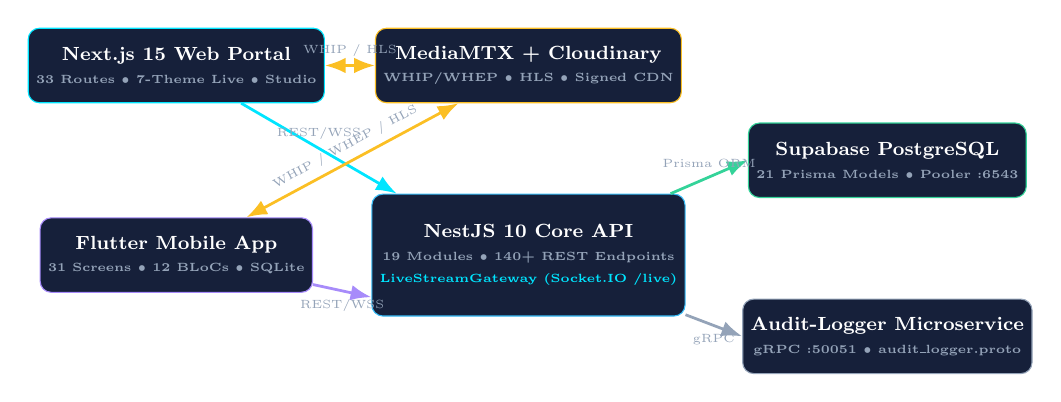
\begin{tikzpicture}[scale=0.86, every node/.style={transform shape, align=center}]
    \node[draw=omniCyan, fill=omniCard, rounded corners=4pt, text=white, font=\footnotesize\bfseries, minimum width=38mm, minimum height=11mm] (web) at (0, 2.2) {Next.js 15 Web Portal\\{\tiny\color{omniSlate}33 Routes $\bullet$ 7-Theme Live $\bullet$ Studio}};
    \node[draw=omniPurple, fill=omniCard, rounded corners=4pt, text=white, font=\footnotesize\bfseries, minimum width=38mm, minimum height=11mm] (mob) at (0, -0.6) {Flutter Mobile App\\{\tiny\color{omniSlate}31 Screens $\bullet$ 12 BLoCs $\bullet$ SQLite}};

    \node[draw=omniAmber, fill=omniCard, rounded corners=4pt, text=white, font=\footnotesize\bfseries, minimum width=34mm, minimum height=11mm] (mtx) at (5.2, 2.2) {MediaMTX + Cloudinary\\{\tiny\color{omniSlate}WHIP/WHEP $\bullet$ HLS $\bullet$ Signed CDN}};

    \node[draw=omniBlue, fill=omniCard, rounded corners=4pt, text=white, font=\footnotesize\bfseries, minimum width=42mm, minimum height=18mm] (api) at (5.2, -0.6) {NestJS 10 Core API\\{\tiny\color{omniSlate}19 Modules $\bullet$ 140+ REST Endpoints}\\{\tiny\color{omniCyan}LiveStreamGateway (Socket.IO /live)}};

    \node[draw=omniGreen, fill=omniCard, rounded corners=4pt, text=white, font=\footnotesize\bfseries, minimum width=35mm, minimum height=11mm] (db) at (10.5, 0.8) {Supabase PostgreSQL\\{\tiny\color{omniSlate}21 Prisma Models $\bullet$ Pooler :6543}};
    \node[draw=omniSlate, fill=omniCard, rounded corners=4pt, text=white, font=\footnotesize\bfseries, minimum width=35mm, minimum height=11mm] (grpc) at (10.5, -1.8) {Audit-Logger Microservice\\{\tiny\color{omniSlate}gRPC :50051 $\bullet$ audit\_logger.proto}};

    \draw[-{Latex}, omniCyan, line width=1pt] (web) -- node[above, font=\tiny, text=omniSlate]{REST/WSS} (api.155);
    \draw[-{Latex}, omniPurple, line width=1pt] (mob) -- node[below, font=\tiny, text=omniSlate]{REST/WSS} (api.195);
    \draw[{Latex}-{Latex}, omniAmber, line width=1pt] (web) -- node[above, font=\tiny, text=omniSlate]{WHIP / HLS} (mtx);
    \draw[{Latex}-{Latex}, omniAmber, line width=1pt] (mob) -- node[above, font=\tiny, text=omniSlate, sloped]{WHIP / WHEP / HLS} (mtx);
    \draw[-{Latex}, omniGreen, line width=1pt] (api) -- node[above, font=\tiny, text=omniSlate]{Prisma ORM} (db.west);
    \draw[-{Latex}, omniSlate, line width=1pt] (api) -- node[below, font=\tiny, text=omniSlate]{gRPC} (grpc.west);
  \end{tikzpicture}
  \end{center}
  \vspace*{-2mm}
  \begin{center}
    \tiny\color{omniSlate}A unified monorepo architecture developed at \textbf{FPTU Quy Nhon AI Campus --- FU Cahata} under Mentor \textbf{Mr. Huỳnh Vang}.
  \end{center}
\end{frame}

% ============================================================
% SLIDE 5: End-to-End LiveStream & Live Studio Real-Time Architecture
% ============================================================
\begin{frame}{LiveStream \& Live Studio Architecture}{Bi-Directional WebRTC WHIP/WHEP, MediaMTX HLS \& Socket.IO \texttt{/live} Pipeline}
  \begin{center}
  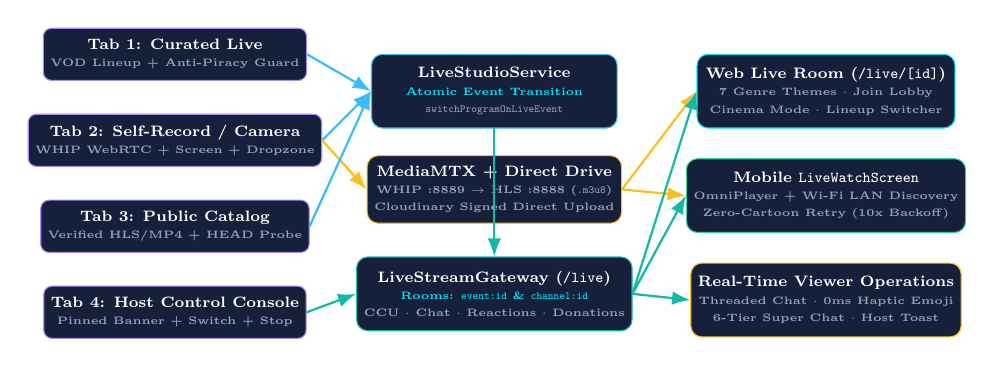
\begin{tikzpicture}[scale=0.78, every node/.style={transform shape, align=center}]
    % Left: 4 Studio Modes
    \node[draw=omniPurple, fill=omniCard, rounded corners=3pt, text=white, font=\scriptsize\bfseries, minimum width=36mm, minimum height=8.5mm] (t1) at (0, 2.4) {Tab 1: Curated Live\\{\tiny\color{omniSlate}VOD Lineup + Anti-Piracy Guard}};
    \node[draw=omniPurple, fill=omniCard, rounded corners=3pt, text=white, font=\scriptsize\bfseries, minimum width=36mm, minimum height=8.5mm] (t2) at (0, 1.0) {Tab 2: Self-Record / Camera\\{\tiny\color{omniSlate}WHIP WebRTC + Screen + Dropzone}};
    \node[draw=omniPurple, fill=omniCard, rounded corners=3pt, text=white, font=\scriptsize\bfseries, minimum width=36mm, minimum height=8.5mm] (t3) at (0,-0.4) {Tab 3: Public Catalog\\{\tiny\color{omniSlate}Verified HLS/MP4 + HEAD Probe}};
    \node[draw=omniPurple, fill=omniCard, rounded corners=3pt, text=white, font=\scriptsize\bfseries, minimum width=36mm, minimum height=8.5mm] (t4) at (0,-1.8) {Tab 4: Host Control Console\\{\tiny\color{omniSlate}Pinned Banner + Switch + Stop}};

    % Middle: Orchestration
    \node[draw=omniBlue, fill=omniCard, rounded corners=4pt, text=white, font=\scriptsize\bfseries, minimum width=40mm, minimum height=12mm] (svc) at (5.2, 1.8) {LiveStudioService\\{\tiny\color{omniCyan}Atomic Event Transition}\\{\tiny\color{omniSlate}\texttt{switchProgramOnLiveEvent}}};
    \node[draw=omniAmber, fill=omniCard, rounded corners=4pt, text=white, font=\scriptsize\bfseries, minimum width=40mm, minimum height=11mm] (media) at (5.2, 0.2) {MediaMTX + Direct Drive\\{\tiny\color{omniSlate}WHIP :8889 $\rightarrow$ HLS :8888 (\texttt{.m3u8})}\\{\tiny\color{omniSlate}Cloudinary Signed Direct Upload}};
    \node[draw=omniTeal, fill=omniCard, rounded corners=4pt, text=white, font=\scriptsize\bfseries, minimum width=40mm, minimum height=12mm] (gw) at (5.2,-1.5) {LiveStreamGateway (\texttt{/live})\\{\tiny\color{omniCyan}Rooms: \texttt{event:id} \& \texttt{channel:id}}\\{\tiny\color{omniSlate}CCU $\cdot$ Chat $\cdot$ Reactions $\cdot$ Donations}};

    % Right: Viewer Rooms
    \node[draw=omniCyan, fill=omniCard, rounded corners=4pt, text=white, font=\scriptsize\bfseries, minimum width=42mm, minimum height=12mm] (wroom) at (10.6, 1.8) {Web Live Room (\texttt{/live/[id]})\\{\tiny\color{omniSlate}7 Genre Themes $\cdot$ Join Lobby}\\{\tiny\color{omniSlate}Cinema Mode $\cdot$ Lineup Switcher}};
    \node[draw=omniGreen, fill=omniCard, rounded corners=4pt, text=white, font=\scriptsize\bfseries, minimum width=42mm, minimum height=12mm] (mroom) at (10.6, 0.1) {Mobile \texttt{LiveWatchScreen}\\{\tiny\color{omniSlate}OmniPlayer + Wi-Fi LAN Discovery}\\{\tiny\color{omniSlate}Zero-Cartoon Retry (10x Backoff)}};
    \node[draw=omniAmber, fill=omniCard, rounded corners=4pt, text=white, font=\scriptsize\bfseries, minimum width=42mm, minimum height=12mm] (ops) at (10.6,-1.6) {Real-Time Viewer Operations\\{\tiny\color{omniSlate}Threaded Chat $\cdot$ 0ms Haptic Emoji}\\{\tiny\color{omniSlate}6-Tier Super Chat $\cdot$ Host Toast}};

    \draw[-{Latex}, omniBlue, line width=0.8pt] (t1.east) -- (svc.west);
    \draw[-{Latex}, omniBlue, line width=0.8pt] (t2.east) -- (svc.west);
    \draw[-{Latex}, omniAmber, line width=0.8pt] (t2.east) -- (media.west);
    \draw[-{Latex}, omniBlue, line width=0.8pt] (t3.east) -- (svc.west);
    \draw[-{Latex}, omniTeal, line width=0.8pt] (t4.east) -- (gw.west);
    \draw[-{Latex}, omniTeal, line width=0.8pt] (svc) -- (gw);
    \draw[-{Latex}, omniAmber, line width=0.8pt] (media.east) -- (wroom.west);
    \draw[-{Latex}, omniAmber, line width=0.8pt] (media.east) -- (mroom.west);
    \draw[-{Latex}, omniTeal, line width=0.8pt] (gw.east) -- (wroom.west);
    \draw[-{Latex}, omniTeal, line width=0.8pt] (gw.east) -- (mroom.west);
    \draw[-{Latex}, omniTeal, line width=0.8pt] (gw.east) -- (ops.west);
  \end{tikzpicture}
  \end{center}
\end{frame}

% ============================================================
% PART 1 DIVIDER
% ============================================================
\section{PRN232 Back-End \& Web}
{
\setbeamertemplate{headline}{}
\begin{frame}[plain]
  \begin{tikzpicture}[remember picture, overlay]
    \fill[omniDeep] (current page.north west) rectangle (current page.south east);
    \fill[omniBlue!10] ($(current page.north west) + (0,-15mm)$) rectangle ($(current page.south east) + (0,15mm)$);
  \end{tikzpicture}
  \begin{center}
    \vspace{10mm}
    {\scriptsize\bfseries\color{omniCyan}MODULE 1 OF 2 $\bullet$ FPTU QUY NHON AI CAMPUS --- FU CAHATA}\\[3mm]
    {\Huge\bfseries\color{white}PART 1: PRN232}\\[3mm]
    {\Large\bfseries\color{omniBlue}Building Cross-Platform Back-End Application \& Web Portal}\\[4mm]
    {\color{omniBorder}\rule{0.5\linewidth}{1pt}}\\[4mm]
    {\footnotesize\color{omniSlate}NestJS 10 $\bullet$ Next.js 15 (33 Routes) $\bullet$ Live Studio \& Live Room $\bullet$ Supabase PostgreSQL $\bullet$ gRPC $\bullet$ AI Curator}
  \end{center}
\end{frame}
}

% ============================================================
% SLIDE 6: PRN232 Backend Modular Design, RBAC & 5-Domain DB
% ============================================================
\begin{frame}{Backend Architecture, Security \& 5-Domain Database}{NestJS 10 (19 Modules), 4-Role RBAC \& 21 Prisma Models}
  \begin{columns}[t]
    \begin{column}{0.48\textwidth}
      \card{\linewidth}{omniBlue}{19 MODULES \& 5-DOMAIN DATABASE (21 MODELS)}{
        \begin{itemize}
          \setlength\itemsep{1mm}
          \item \textbf{1. Identity \& Security:} \texttt{User}, \texttt{Role}, \texttt{RefreshToken}, \texttt{PasswordResetToken} (JWT 60m + 90d rotation).
          \item \textbf{2. Broadcast Core:} \texttt{LiveChannel}, \texttt{LiveEvent}, \texttt{Recording}, \texttt{ProductionTag}.
          \item \textbf{3. Social \& Live Monetization:} \texttt{Comment}, \texttt{CommentLike}, \texttt{Reaction}, \texttt{Follow}, \texttt{Watchlist}, \texttt{WatchHistory}, \texttt{StreamDonation}.
          \item \textbf{4. Operations \& gRPC Audit:} \texttt{AuditLog}, \texttt{Notification}, \texttt{DeviceToken}, \texttt{NewsletterSubscriber}.
          \item \textbf{5. AI Intelligence:} \texttt{AiCuratorReport} (1-to-1 with provenance).
        \end{itemize}
      }
    \end{column}

    \begin{column}{0.48\textwidth}
      \card{\linewidth}{omniTeal}{SECURITY PIPELINE \& RBAC MATRIX}{
        \begin{itemize}
          \setlength\itemsep{1.2mm}
          \item \textbf{Role-Based Access Control (4 Roles):}
            \begin{itemize}
              \item \texttt{ADMIN}: System governance, user RBAC, gRPC audit log explorer.
              \item \texttt{STAFF}: Live Studio 4-mode broadcasting, on-the-fly program switch, AI curation, schedule management.
              \item \texttt{VIEWER}: Live room chat, floating reactions, 6-tier Super Chat donations, watchlist \& history.
              \item \texttt{GUEST}: Public EPG grid, channel catalog \& VOD discovery.
            \end{itemize}
          \item \textbf{Defense in Depth:} Helmet, CORS whitelist, Bcrypt (12 rounds), \texttt{safe-log} secret redaction.
        \end{itemize}
      }
    \end{column}
  \end{columns}
\end{frame}

% ============================================================
% SLIDE 7: Algorithmic Core 1 & 2 - Airtime Collision & 24/7 EPG
% ============================================================
\begin{frame}{Algorithmic Core: Collision Prevention \& 24/7 EPG Filler}{Raw SQL Effective-End Interval Check \& Seeded Deterministic Playout}
  \begin{columns}[t]
    \begin{column}{0.50\textwidth}
      \card{\linewidth}{omniCyan}{1. ATOMIC SQL SCHEDULE CONFLICT DETECTION}{
        Two broadcasts $A$ and $B$ collide iff $\max(\text{start}_A, \text{start}_B) < \min(\text{end}_A, \text{end}_B)$.
        \begin{tcolorbox}[colback=omniDark, colframe=omniBorder, boxrule=0.5pt, arc=2pt, left=2mm, right=2mm, top=1mm, bottom=1mm]
        \tiny\ttfamily\color{omniCyan}
        SELECT id, title FROM "LiveEvent"\\
        WHERE "channelId" = \$1::uuid\\
        \ \ AND status IN ('SCHEDULED', 'LIVE')\\
        \ \ AND "scheduledAt" < \$newEnd\\
        \ \ AND COALESCE("endedAt",\\
        \ \ \ \ "scheduledAt" + ("duration" || ' min')::interval)\\
        \ \ \ \ > \$newStart;
        \end{tcolorbox}
        {\scriptsize\color{omniSlate}$\bullet$ Handles \texttt{NULL endedAt} on active events and returns HTTP \texttt{409 Conflict} with colliding event details.}
      }
    \end{column}

    \begin{column}{0.46\textwidth}
      \card{\linewidth}{omniPurple}{2. SEEDED 24/7 EPG AUTO-FILLER ENGINE}{
        \begin{itemize}
          \setlength\itemsep{1.2mm}
          \item \textbf{Zero Empty Days:} Guarantees full 24-hour (00:00--23:59) coverage for every channel and date.
          \item \textbf{Seeded PRNG:} Keyed on \texttt{(date, channelId)} so every client renders the exact same schedule.
          \item \textbf{Genre-Aware \& Episode Splitting:} Prioritizes matching channel category, splits long VODs into episodes, and caps daily repeats (\texttt{MAX\_REPEATS\_PER\_ITEM\_PER\_DAY}).
          \item \textbf{Pure Function:} Zero I/O side effects, verified by 18 unit tests.
        \end{itemize}
      }
    \end{column}
  \end{columns}
\end{frame}

% ============================================================
% SLIDE 8: Algorithmic Core 3 - Enterprise AI Curator & gRPC Audit
% ============================================================
\begin{frame}{AI Broadcast Curator \& gRPC Audit Microservice}{Single-Call GPT-4o + Zod Schema Validation + Binary HTTP/2 gRPC Telemetry}
  \begin{columns}[c]
    \begin{column}{\textwidth}
      \centering
      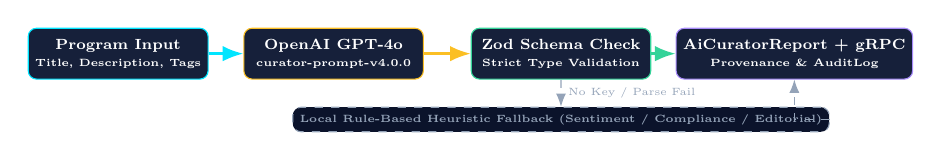
\begin{tikzpicture}[scale=0.76, every node/.style={transform shape, align=center}]
        \node[draw=omniCyan, fill=omniCard, rounded corners=3pt, font=\scriptsize\bfseries, text=white, minimum width=26mm, minimum height=8.5mm] (in) at (0,0) {Program Input\\{\tiny Title, Description, Tags}};
        \node[draw=omniAmber, fill=omniCard, rounded corners=3pt, font=\scriptsize\bfseries, text=white, minimum width=30mm, minimum height=8.5mm] (llm) at (3.6,0) {OpenAI GPT-4o\\{\tiny curator-prompt-v4.0.0}};
        \node[draw=omniGreen, fill=omniCard, rounded corners=3pt, font=\scriptsize\bfseries, text=white, minimum width=30mm, minimum height=8.5mm] (zod) at (7.4,0) {Zod Schema Check\\{\tiny Strict Type Validation}};
        \node[draw=omniPurple, fill=omniCard, rounded corners=3pt, font=\scriptsize\bfseries, text=white, minimum width=32mm, minimum height=8.5mm] (audit) at (11.3,0) {AiCuratorReport + gRPC\\{\tiny Provenance \& AuditLog}};

        \draw[-{Latex}, omniCyan, line width=1pt] (in) -- (llm);
        \draw[-{Latex}, omniAmber, line width=1pt] (llm) -- (zod);
        \draw[-{Latex}, omniGreen, line width=1pt] (zod) -- (audit);

        \node[draw=omniSlate, dashed, fill=omniDark, rounded corners=3pt, font=\tiny\bfseries, text=omniSlate] (fall) at (7.4,-1.1) {Local Rule-Based Heuristic Fallback (Sentiment / Compliance / Editorial)};
        \draw[-{Latex}, omniSlate, dashed] (zod) -- node[right, font=\tiny]{No Key / Parse Fail} (fall);
        \draw[-{Latex}, omniSlate, dashed] (fall) -| (audit);
      \end{tikzpicture}
    \end{column}
  \end{columns}
  \vspace{1mm}
  \begin{columns}[t]
    \begin{column}{0.48\textwidth}
      \card{\linewidth}{omniGreen}{CONSOLIDATED AI CURATOR (\texttt{v4.0.0})}{
        \begin{itemize}
          \setlength\itemsep{0.8mm}
          \item Merges description, tags, compliance \& suitability into 1 LLM call (\texttt{temp=0.3}, \texttt{top\_p=0.95}), cutting latency by 66\%.
          \item Records \texttt{promptVersion}, \texttt{aiModelVersion}, \texttt{openaiCallMs} and \texttt{openaiRetries}.
        \end{itemize}
      }
    \end{column}
    \begin{column}{0.48\textwidth}
      \card{\linewidth}{omniPurple}{STANDALONE gRPC AUDIT MICROSERVICE}{
        \begin{itemize}
          \setlength\itemsep{0.8mm}
          \item Exposes \texttt{LogAudit}, \texttt{GetLogsByUser}, \texttt{GetLogsByAction}, \texttt{GetLogsByEntity}, \texttt{GetLogStats} over port \texttt{50051}.
          \item Non-blocking fire-and-forget RPC keeps main API latency unaffected.
        \end{itemize}
      }
    \end{column}
  \end{columns}
\end{frame}

% ============================================================
% SLIDE 9: Web Portal (33 Routes), Live Room (/live/[id]) & Studio (/studio/live)
% ============================================================
\begin{frame}{Next.js 15 Web Portal: LiveStream Room \& Live Studio}{33 Routes, 7 Genre-Themed Live Lounges \& 4-Tab Broadcast Control Console}
  \begin{columns}[t]
    \begin{column}{0.48\textwidth}
      \card{\linewidth}{omniCyan}{INTERACTIVE LIVESTREAM ROOM (\texttt{/live} \& \texttt{/live/[id]})}{
        \begin{itemize}
          \setlength\itemsep{1mm}
          \item \textbf{Live Hub (\texttt{/live}):} Auto-refreshes every 15s, displays total LIVE events \& aggregate CCU pills, trending/newest sort.
          \item \textbf{7 Genre-Themed Lounges:} Dynamically styles room into \emph{Kids}, \emph{Podcast}, \emph{Music Stage}, \emph{Academy}, \emph{Sports Arena}, \emph{Obsidian Theater} or \emph{Broadcast Lounge}.
          \item \textbf{Viewer Operations:} \texttt{JoinLobbyCard} entry, \textbf{Cinema Mode} (lights-off focus), multi-item \textbf{lineup program switcher}, real-time Socket.IO chat, \textbf{4 floating reactions} ($\heartsuit$, Fire, Clap, Wow) \& pinned host banner.
        \end{itemize}
      }
    \end{column}

    \begin{column}{0.48\textwidth}
      \card{\linewidth}{omniBlue}{4-TAB WEB LIVE STUDIO CONSOLE (\texttt{/studio/live})}{
        \begin{itemize}
          \setlength\itemsep{1mm}
          \item \textbf{Tab 1 (Curated Live):} Pick 1 or more VOD recordings (\texttt{lineup}) with Anti-Piracy Guard \& atomic transition.
          \item \textbf{Tab 2 (Camera / Screen / Upload):} \texttt{WebcamLiveBroadcaster} (WebRTC WHIP to MediaMTX), Screen Share (\texttt{getDisplayMedia}), or \texttt{UploadDropzone} (Signed Direct-to-Cloudinary upload with speed/ETA \& canvas thumbnail).
          \item \textbf{Tab 3 (Verified Public Catalog):} 1-click import of verified HLS/MP4 streams with server \texttt{HEAD} probe.
          \item \textbf{Tab 4 (Host Console):} Broadcast pinned announcements (\texttt{broadcaster:message}) \& stop live (\texttt{keepAsVod}).
        \end{itemize}
      }
    \end{column}
  \end{columns}
\end{frame}

% ============================================================
% PART 2 DIVIDER
% ============================================================
\section{PRM393 Mobile Client}
{
\setbeamertemplate{headline}{}
\begin{frame}[plain]
  \begin{tikzpicture}[remember picture, overlay]
    \fill[omniDeep] (current page.north west) rectangle (current page.south east);
    \fill[omniPurple!10] ($(current page.north west) + (0,-15mm)$) rectangle ($(current page.south east) + (0,15mm)$);
  \end{tikzpicture}
  \begin{center}
    \vspace{10mm}
    {\scriptsize\bfseries\color{omniCyan}MODULE 2 OF 2 $\bullet$ FPTU QUY NHON AI CAMPUS --- FU CAHATA}\\[3mm]
    {\Huge\bfseries\color{white}PART 2: PRM393}\\[3mm]
    {\Large\bfseries\color{omniPurple}Mobile Applications Development (Flutter 3.x \& Dart)}\\[4mm]
    {\color{omniBorder}\rule{0.5\linewidth}{1pt}}\\[4mm]
    {\footnotesize\color{omniSlate}31 Screens $\bullet$ 12 BLoCs $\bullet$ OmniPlayer + LAN Discovery $\bullet$ Mobile Live Studio \& Recorder $\bullet$ Offline SQLite}
  \end{center}
\end{frame}
}

% ============================================================
% SLIDE 11: Mobile Architecture & 31-Screen Hierarchy
% ============================================================
\begin{frame}{Mobile Clean Architecture \& 31-Screen Hierarchy}{4-Tier Clean Architecture, 12 BLoC/Cubits \& Declarative GoRouter Topology}
  \begin{columns}[t]
    \begin{column}{0.48\textwidth}
      \card{\linewidth}{omniPurple}{4-TIER CLEAN ARCHITECTURE \& 12 BLOCS}{
        \begin{itemize}
          \setlength\itemsep{1mm}
          \item \textbf{Presentation (31 Screens, 22 Widgets):} 6-tab \texttt{MainNavigationShell} (\texttt{Home}, \texttt{Channels}, \texttt{Schedule}, \texttt{Saved}, \texttt{History}, \texttt{Profile}) + Auth, Live, Studio \& Admin clusters.
          \item \textbf{Logic (12 BLoC/Cubits):} \texttt{AuthBloc}, \texttt{ChannelBloc}, \texttt{EpgBloc}, \texttt{WatchlistBloc}, \texttt{LiveEventsCubit}, \texttt{ThemeCubit}, \texttt{LanguageCubit} with \texttt{droppable}/\texttt{restartable} transformers.
          \item \textbf{Data \& Core:} 10 Repositories, Dio \texttt{AuthInterceptor} (401 queue lock \& refresh), SQLite \texttt{omnicast\_local.db}.
        \end{itemize}
      }
    \end{column}

    \begin{column}{0.48\textwidth}
      \card{\linewidth}{omniGreen}{OFFLINE-FIRST SQLITE \& LOCAL ALARMS}{
        \begin{itemize}
          \setlength\itemsep{1mm}
          \item \textbf{Offline Watchlist \& EPG Cache:} Reads seamlessly from local SQLite when network drops.
          \item \textbf{Pending Mutation Queue (\texttt{pending\_ops}):} Queues offline add/remove actions and replays FIFO upon reconnection.
          \item \textbf{15-Minute Advance Reminders:} Schedules exact local OS notifications 15 minutes before a bookmarked show airs.
        \end{itemize}
      }
    \end{column}
  \end{columns}
\end{frame}

% ============================================================
% SLIDE 12: Mobile LiveWatchScreen, OmniPlayer & LAN Host Discovery
% ============================================================
\begin{frame}{Mobile LiveStream Experience: \texttt{LiveWatchScreen} \& \texttt{OmniPlayer}}{Wi-Fi LAN Host Discovery, Zero-Cartoon Retry \& 6 Interactive Live Operations}
  \begin{columns}[t]
    \begin{column}{0.48\textwidth}
      \card{\linewidth}{omniAmber}{MULTI-ENGINE \texttt{OmniPlayer} \& LAN DISCOVERY}{
        \begin{itemize}
          \setlength\itemsep{1mm}
          \item \textbf{Automatic Wi-Fi LAN Discovery (\texttt{LanDiscoveryService}):} Scans the local \texttt{/24} subnet on port \texttt{8888} to auto-replace \texttt{localhost}/\texttt{10.0.2.2} with the real MediaMTX host IP on physical phones.
          \item \textbf{Zero-Cartoon-Fallback Live Retry:} For live camera feeds (\texttt{/live/webcam\_*}), performs up to 10 exponential-backoff retries without falling back to sample VODs.
          \item \textbf{Direct Drive \& VIP Paywall:} Rewrites Google Drive URLs to \texttt{drive.usercontent.google.com} and enforces \texttt{SubscriptionPaymentSheet} on VIP streams.
        \end{itemize}
      }
    \end{column}

    \begin{column}{0.48\textwidth}
      \card{\linewidth}{omniCyan}{\texttt{LiveWatchScreen} (\texttt{/live/:id}) OPERATIONS}{
        \begin{itemize}
          \setlength\itemsep{1mm}
          \item \textbf{1. Lobby \& Live CCU:} \texttt{LiveJoinPromptBanner} + real-time \texttt{live:viewerCount} badge.
          \item \textbf{2. Threaded Live Chat \& Moderation:} Nested replies (\texttt{parentId}), comment likes \& instant \texttt{STAFF}/\texttt{ADMIN} deletion (\texttt{chat:delete}).
          \item \textbf{3. 0ms Haptic Floating Reactions:} \texttt{HapticFeedback.lightImpact()} + optimistic delta + rising particle overlay ($\heartsuit$, Fire, Clap, Wow/Party).
          \item \textbf{4. 6-Tier Super Chat (\texttt{LiveDonationModal}):} Preset gift tiers, custom message \& celebratory banner.
          \item \textbf{5. Pinned Host Toast \& Instant Program Switch:} Handles \texttt{broadcaster:message} \& \texttt{live:program:changed}.
        \end{itemize}
      }
    \end{column}
  \end{columns}
\end{frame}

% ============================================================
% SLIDE 13: Mobile Live Studio (4 Tabs) & MobileStudioRecorderScreen
% ============================================================
\begin{frame}{Mobile Live Studio \& Field Reporter Camera Viewfinder}{\texttt{LiveStudioScreen} (4 Tabs) \& \texttt{MobileStudioRecorderScreen} (WebRTC WHIP)}
  \begin{columns}[t]
    \begin{column}{0.48\textwidth}
      \card{\linewidth}{omniPurple}{\texttt{LiveStudioScreen} (4 BROADCAST TABS)}{
        \begin{itemize}
          \setlength\itemsep{1.2mm}
          \item \textbf{Tab 1 --- Curated Live:} Select channel, title/description, and pick 1 or more VOD recordings (\texttt{lineup}) to go live immediately.
          \item \textbf{Tab 2 --- Self-Record \& Upload:} Launch \texttt{MobileStudioRecorderScreen} or upload device video to Cloudinary via signed parameters (\texttt{IMMEDIATE}, \texttt{SCHEDULED}, \texttt{PRIVATE}).
          \item \textbf{Tab 3 --- Verified Public Catalog:} Browse \& 1-click import verified HLS/MP4 streams or custom URLs.
          \item \textbf{Tab 4 --- Host Console:} Send pinned announcements (\texttt{broadcaster:message}) \& stop active broadcast (\texttt{keepAsVod}).
        \end{itemize}
      }
    \end{column}

    \begin{column}{0.48\textwidth}
      \card{\linewidth}{omniGreen}{\texttt{MobileStudioRecorderScreen} VIEWFINDER}{
        \begin{itemize}
          \setlength\itemsep{1.2mm}
          \item \textbf{Dual Broadcast Modes:}
            \begin{itemize}
              \item \texttt{Push-to-Live}: Real-time WebRTC WHIP streaming via \texttt{WebRTCPublisherService} with flashing red \texttt{ON-AIR} tally border.
              \item \texttt{Record-then-Live}: 1080p MP4 capture + post-record \textbf{Master QC Review} player.
            \end{itemize}
          \item \textbf{Professional Broadcast HUD:} Real-time \textbf{SMPTE Timecode} (\texttt{HH:MM:SS:FF}), dual-channel \textbf{Stereo VU Audio Meter}, \textbf{Rule-of-Thirds} \& \textbf{Safe Area} guides, \textbf{Lower Third} overlay, \texttt{1x--5x} zoom, torch \& auto-scrolling \textbf{Reporter Teleprompter HUD}.
        \end{itemize}
      }
    \end{column}
  \end{columns}
\end{frame}

% ============================================================
% PART 3: SYNERGY, VERIFICATION & DEPLOYMENT
% ============================================================
\section{Synergy \& Verification}
\begin{frame}{Cross-Platform Synergy \& Verification Matrix}{142,897 Physical LOC $\bullet$ 482/482 Automated Tests (100\% Pass)}
  \begin{center}
  \footnotesize
  \renewcommand{\arraystretch}{1.18}
  \begin{tabularx}{0.96\linewidth}{lXX}
    \toprule
    \textbf{Dimension} & \textbf{\color{omniCyan}PRN232 (Back-End, gRPC \& Web)} & \textbf{\color{omniPurple}PRM393 (Flutter Mobile Client)} \\
    \midrule
    \textbf{Core Stack} & NestJS 10 + gRPC + Next.js 15 (33 Routes) & Flutter 3.x + Dart 3 (31 Screens, 22 Widgets) \\
    \textbf{Architecture} & 19 Domain Modules + Standalone gRPC Service & 4-Tier Clean Architecture + 12 BLoC/Cubits \\
    \textbf{Database / Cache} & Supabase PostgreSQL (21 Prisma models) & SQLite (\texttt{omnicast\_local.db} + \texttt{pending\_ops}) \\
    \textbf{LiveStream \& Studio} & 7-Theme Live Room + 4-Tab Web Studio (WHIP) & \texttt{LiveWatchScreen} + 4-Tab Studio + ENG Recorder \\
    \textbf{Realtime Operations} & Socket.IO \texttt{/live}: Chat, Emoji, Super Chat, Switch & 0ms Haptic Emoji, 6-Tier Super Chat, LAN Scan \\
    \textbf{Code Volume} & \textbf{79,568 Physical LOC} & \textbf{53,922 Physical LOC} (+ 9,407 Ops/Docs) \\
    \textbf{Automated Tests} & \textbf{391 Tests} (163 Backend + 228 Web Vitest) & \textbf{91 Tests} (56 Unit + 35 Widget Tests) \\
    \textbf{Pass Rate} & \textbf{\color{omniGreen}100\% PASS} (+ 8 Playwright E2E) & \textbf{\color{omniGreen}100\% PASS} \\
    \bottomrule
  \end{tabularx}
  \end{center}
  \vspace*{-1mm}
  \begin{center}
    \scriptsize\color{omniGreen}\textbf{TOTAL SYSTEM SCALE: 142,897 Lines of Code $\bullet$ 482/482 Automated Tests PASS $\bullet$ Live on Vercel \& Supabase}
  \end{center}
\end{frame}

% ============================================================
% SLIDE 15: Live Production Deployment & Demo Accounts
% ============================================================
\begin{frame}{Live Deployment \& Evaluation}{Production Cloud Infrastructure \& Pre-Seeded Test Credentials}
  \begin{columns}[t]
    \begin{column}{0.52\textwidth}
      \card{\linewidth}{omniBlue}{LIVE PRODUCTION ENDPOINTS}{
        \begin{itemize}
          \setlength\itemsep{1.2mm}
          \item \textbf{Web Portal (Vercel Live):}\\
            \href{https://omnicast-fe.vercel.app}{\color{omniCyan}\texttt{https://omnicast-fe.vercel.app}}
          \item \textbf{Core API Swagger Documentation:}\\
            \href{https://omnicast-api.vercel.app/swagger}{\color{omniCyan}\texttt{https://omnicast-api.vercel.app/swagger}}
          \item \textbf{Mobile APK Release (v1.2.0):}\\
            \texttt{github.com/TomOutfit/.../releases/tag/v1.2.0}
          \item \textbf{Official GitHub Repository:}\\
            \texttt{github.com/TomOutfit/OmniCast\_PRN232-PRM393...}
        \end{itemize}
      }
    \end{column}

    \begin{column}{0.44\textwidth}
      \card{\linewidth}{omniGreen}{PRE-CONFIGURED EVALUATION ACCOUNTS}{
        \textbf{Password for all test accounts:} \texttt{Admin123!}
        \vspace{2mm}
        \begin{itemize}
          \setlength\itemsep{1.5mm}
          \item \textbf{Admin Account (Full RBAC):}\\
            \texttt{admin@omnicast.tv}
          \item \textbf{Staff Account (Live Studio Broadcaster):}\\
            \texttt{staff@omnicast.tv}
          \item \textbf{Viewer Account (Live Chat \& Super Chat):}\\
            \texttt{viewer1@omnicast.tv}
        \end{itemize}
      }
    \end{column}
  \end{columns}
\end{frame}

% ============================================================
% SLIDE 16: Conclusion & Q&A
% ============================================================
\section{Conclusion}
{
\setbeamertemplate{headline}{}
\setbeamertemplate{footline}{}
\begin{frame}[plain]
  \begin{tikzpicture}[remember picture, overlay]
    \fill[omniDeep] (current page.north west) rectangle (current page.south east);
    \draw[omniCyan!30, line width=0.8pt, dashed] ($(current page.north west) + (10mm,-10mm)$) rectangle ($(current page.south east) + (-10mm,10mm)$);
    \draw[omniBorder, line width=1.2pt] ($(current page.north west) + (12mm,-12mm)$) rectangle ($(current page.south east) + (-12mm,12mm)$);
  \end{tikzpicture}
  \begin{center}
    \vspace{4mm}
    {\scriptsize\bfseries\color{omniCyan}FPTU QUY NHON AI CAMPUS --- FU CAHATA $\bullet$ MENTOR: THẦY HUỲNH VANG}\\[2mm]
    {\Huge\bfseries\color{white}Thank You for Your Attention!}\\[2mm]
    {\large\bfseries\color{omniCyan}OmniCast: Enterprise Media \& Broadcast Intelligence Network}\\[3mm]
    {\color{omniBorder}\rule{0.65\linewidth}{1pt}}\\[3mm]

    {\footnotesize\color{white}\textbf{Nguyễn Bình An} \ $\bullet$ \ \textbf{Trần Thanh Sơn} (\texttt{QE170080}) \ $\bullet$ \ \textbf{Nguyễn Vĩnh Phú} (\texttt{QE180136}) \ $\bullet$ \ \textbf{Đồng Hoàng Nguyên}}\\[3mm]
    {\normalsize\bfseries\color{omniAmber}We are ready for Live Demonstration \& Committee Q\&A}\\[4mm]

    
\begin{tikzpicture}
      \node[draw=omniCyan, fill=omniCard, rounded corners=3pt, text=white, font=\scriptsize] (w1) at (-4.2,0) {
        \textbf{Web:} \texttt{omnicast-fe.vercel.app}
      };
      \node[draw=omniPurple, fill=omniCard, rounded corners=3pt, text=white, font=\scriptsize] (w2) at (0,0) {
        \textbf{API:} \texttt{omnicast-api.vercel.app/swagger}
      };
      \node[draw=omniGreen, fill=omniCard, rounded corners=3pt, text=white, font=\scriptsize] (w3) at (4.5,0) {
        \textbf{GitHub:} \texttt{github.com/TomOutfit/OmniCast}
      };
    \end{tikzpicture}
    \vspace{4mm}

    {\scriptsize\color{omniSlate}FPTU Quy Nhon AI Campus --- FU Cahata $\bullet$ Faculty of Information Technology, FPT University $\bullet$ Fall 2026}
  \end{center}
\end{frame}
}

\end{document}
